\documentclass[12pt, twoside]{article}
\usepackage[francais]{babel}
\usepackage[T1]{fontenc}
\usepackage[latin1]{inputenc}
\usepackage[left=5mm, right=5mm, top=3mm, bottom=3mm]{geometry}
\usepackage{float}
\usepackage{graphicx}
\usepackage{array}
\usepackage{multirow}
\usepackage{amsmath,amssymb,mathrsfs}
\usepackage{soul}
\usepackage{textcomp}
\usepackage{eurosym}
 \usepackage{variations}
\usepackage{tabvar}


\pagestyle{empty}

\begin{document}



\section*{\center{Devoir maison 7}}

\begin{center}
\fbox{
\begin{minipage}{19cm}
\textit{Devoir � rendre sur feuille grand format pour le \ul{mercredi 3 avril
2013}. La justification et la \textbf{r�daction} seront prises en
 compte dans le bar�me.}
 \end{minipage}
} 
\end{center}

 
\bigskip

\textbf{\ul{Exercice 1}} \textit{(4 points)} 

\enskip

Le stade du Parc des Cygnes peut contenir 15 000 places. Il y a $x$ places en
virage, les autres en tribune. Les places en virage co�tent 10 \euro, les
places en tribune co�tent 13 \euro. Aujourd'hui, le stade est plein.

\begin{enumerate}
  \item Que repr�sentent les trois expressions suivantes:
 \qquad  $10x$ \qquad \qquad  $15 000-x$ \qquad \qquad  $(15 000-x) \times
  13$
  
  \item Ecrire en fonction de $x$ le montant total de la recette (c'est-�-dire
  la somme d'argent gagn�e par la vente des billets.)
  \item Calculer cette recette si x=6500.
\end{enumerate}


\bigskip

\textbf{\ul{Exercice 2}} \textit{(3 points)}

\enskip

R�duire les expressions suivantes:

$A=2t+4-(8t-9)$ \qquad \qquad $B=3a-7+(2a+5)-(-3a+10)$ \qquad \qquad $C=4y^2-2
\times 3y + 2y \times 5y - 6-4y$


\bigskip



\textbf{\ul{Exercice 3}} \textit{(4 points)}

\begin{tabular}{cc}
\begin{minipage}{9cm}

En utilisant les informations port�es sur la figure:


\begin{enumerate}
  \item Calculer MN.
  \item En d�duire BC.
\end{enumerate} 
\end{minipage}
&
\begin{minipage}{9cm}
\begin{center}
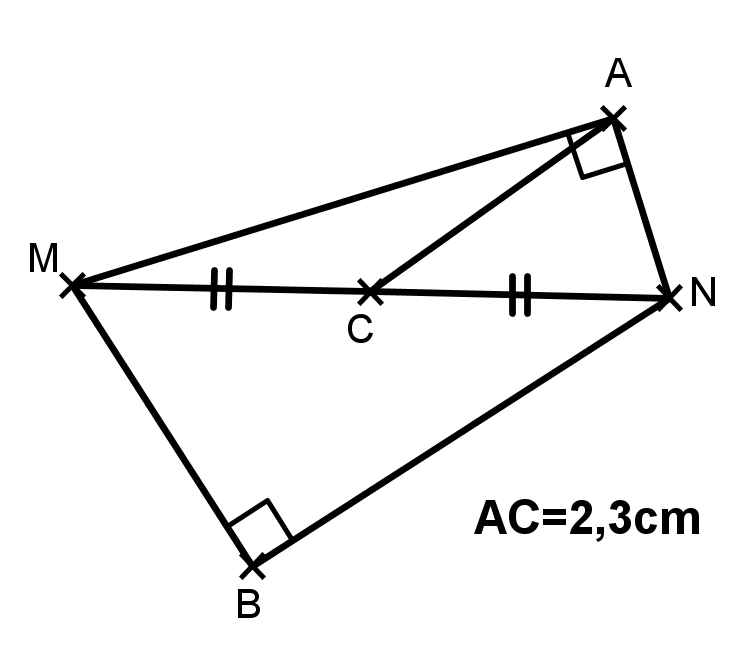
\includegraphics[width=4cm]{images/ex2bis.png}
\end{center}

\end{minipage}
\end{tabular}

\bigskip

\textbf{\ul{Exercice 4}} \textit{(3,5 points)}


\begin{tabular}{cr} 
\begin{minipage}{11cm}

Construire un point P tels que les triangles ABP et CDP soient rectangles en P.
Justifier votre r�ponse.

\enskip

(\textit{La construction se fera sur la photocopie et les explications seront
not�es sur votre feuille.})


\end{minipage}
&
\begin{minipage}{7cm}
\begin{center}
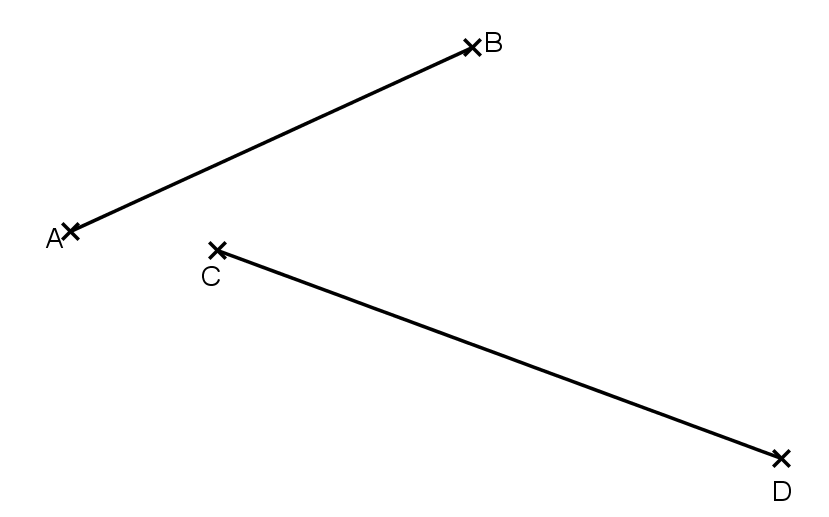
\includegraphics[width=65mm]{images/ex4.png}
\end{center}
\end{minipage} 
\end{tabular}

\bigskip

\textbf{\ul{Exercice 5}} \textit{(5,5 points)}


\enskip

 Soit [IJ] un segment de longueur 8cm. $\mathcal{C}$
est le cercle de diam�tre [IJ]. Le point K appartient au cercle $\mathcal{C}$
et v�rifie JK=3,5cm.



\begin{enumerate}
  \item Faire la figure.
  \item D�montrer que le triangle IJK est rectangle en K.
  \item Calculer JK (on donnera le r�sultat arrondi au mm). Justifier votre
  r�ponse.
  \item Calculer la mesure de l'angle $\widehat{IJK}$. Justifier votre r�ponse.
\end{enumerate}
\end{document}
